\section{Колебания и дифференциальные уравнения}
\epigraph{\textsf{May the force be with you.}}{\texttt{Everybody from SW.}}
Перейдем к кульминации всего курса - составлению дифференциальных уравнений (уравнения на функцию, где фигурирует ее производная), которые являются неотъемлемой частью познания физических законов. Не будем перегонять из пустого в порожнее!
\subsection{Формула Циолковского}


\begin{figure}[h!]
    \centering{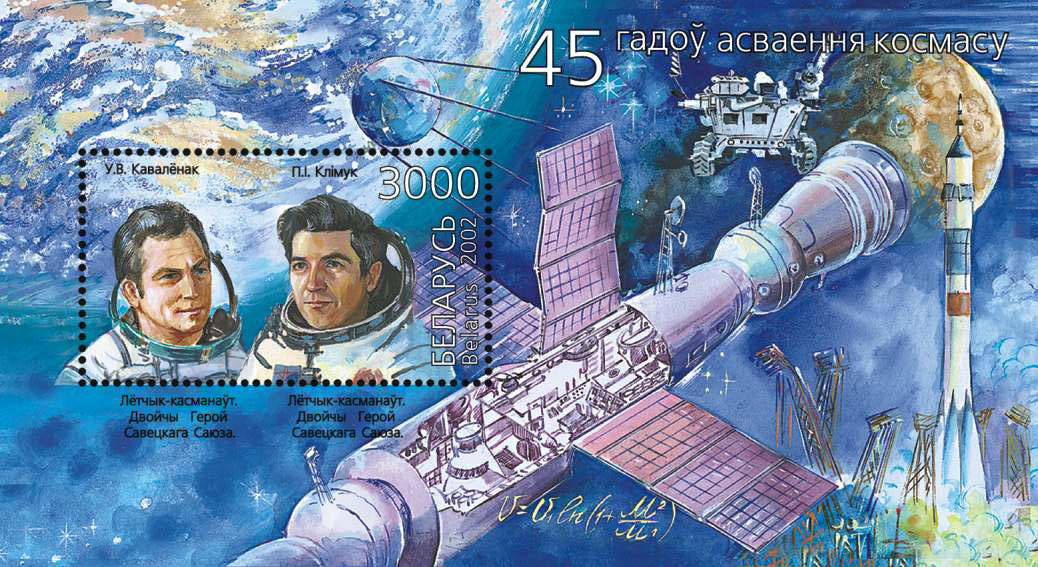
\includegraphics[scale=0.2]{pics/rocket.jpg}}
    \caption{Уравнение Циолковского на марке}
\end{figure}

Рассмотрим движение ракеты в космосе.
Сначала пренебрежём всеми внешними силами, действующими на ракету. Основными параметрами, характеризующими ракету и её двигатель, являются: $\boldsymbol{u}_0$ — скорость истечения газов из сопла ракеты относительно корпуса ракеты, для простоты считаем её постоянной, $M_0$ — исходная масса ракеты с горючим, $M_{\text{к}}$ — конечная масса ракеты после выгорания всего горючего.

Ракета имеет скорость $v$, массу $M$ в момент времени $t$. Выбрасывается топливо массы $\Delta M$ со скоростью $u_0$. Импульс сохраняется, тогда 
\begin{equation*}
    Mv = (M - \Delta M)(v + \Delta v) + \Delta M (v + u_0)
\end{equation*}

Тогда получим
\begin{equation*}
    M\Delta v =  - \Delta M u_0 \Rightarrow v(t) = - u_0 \int_{M}^{M_\text{к}} \frac{dM}{M}
\end{equation*}
Этот сделан предварительно перейдя к дифференциалам. Итого
\begin{equation*}
    v = u_0 \ln \Bigl(\frac{M_0}{M_{\text{к}}} \Bigr)
\end{equation*}
Таким образом, скорость ракеты увеличивается с уменьшением массы ракеты!!! Именно поэтому мы грузим топливо в ракеты, а не просто запускаем их из, например, рогатки.
\subsection{Почему Коши оказался в диффурах?}
Теперь зададимся вопросом - почему дифференциальные уравнения (вообще любые) имеют решения при должном числе условий, наложенных на функцию? Оказывается, что ответ на этот вопрос был дан довольно-таки давно. Задачи, где дано дифференциальное уравнение и условие на функцию, называют \textit{задачами Коши}. Например, уравнение Циолковского
\begin{equation*}
    \begin{cases}
        \frac{dv}{dM}= - \frac{u_0}{M}\\
        v(M = M_0) = 0
    \end{cases}
\end{equation*}

Так оказывается, что такие задачи \textbf{всегда} имеют решение!
\begin{theorem}(Теорема о разрешимости задачи Коши)
    Пусть есть поставленная задача Коши на отрезке
    \begin{equation*}
        \begin{cases}
            y^{'} = f(x,y),\ x \in (x_0, a]\\
            y^{'}(x_0) = y^{0}
        \end{cases}
    \end{equation*}
    Тогда, если функция $f(x,y)$ удовлетворяет (\dots \textbf{куча условий} \dots), то решение \textbf{существует} и \textbf{единственно}.
\end{theorem}
Подробнее об этом вам расскажут в университете, поэтому на этом мы внимание заострять не будем.
\subsection{Математический маятник: чем больше тел, тем сложнее путь}

\subsection{Гармонический осциллятор}
\subsection{Фазовая плоскость}